\chapter{Neural Network}

Imagine a linear classification which computes scores for different visual categories given the image using the formula $s=Wx$, where $W$ is a matrix and $x$ was an input column vector containing all pixel data of the image. In the case of CIFAR-10, $x$ is a $3072 \times 1 $ column vector, and $W$ is a $10 \times 3072$ matrix, so that the output scores is a vector of 10 class scores.

An example neural network would instead compute $s=W_2\max(0,W_1x)$. Here, $W_1$ could be, for example, a $100 \times 3072$ matrix transforming the image into a 100-dimensional intermediate vector. The function $\max(0,−)$ is a non-linearity that is applied elementwise. There are several choices we could make for the non-linearity (which we’ll see later), but this one is a common choice and simply thresholds all activations that are below zero to zero. These are the so called \textit{activation functions}. Finally, the matrix $W_2$ would then be of size $10 \times 100$, so that we again get 10 numbers out that we interpret as the class scores. Notice that the non-linearity is critical computationally - if we left it out, the two matrices could be collapsed to a single matrix, and therefore the predicted class scores would again be a linear function of the input. The non-linearity is where we get the wiggle. The parameters $W_2,W_1$ are learned with stochastic gradient descent, and their gradients are derived with chain rule (and computed with backpropagation).

A three-layer neural network could analogously look like $s=W_3\max(0,W_2\max(0,W_1x))$, where all of $W_3,W_2,W_1$ are parameters to be learned. The sizes of the intermediate hidden vectors are hyperparameters of the network and we’ll see how we can set them later. Lets now look into how we can interpret these computations from the neuron/network perspective.

\begin{figure}[h]
  \centering
  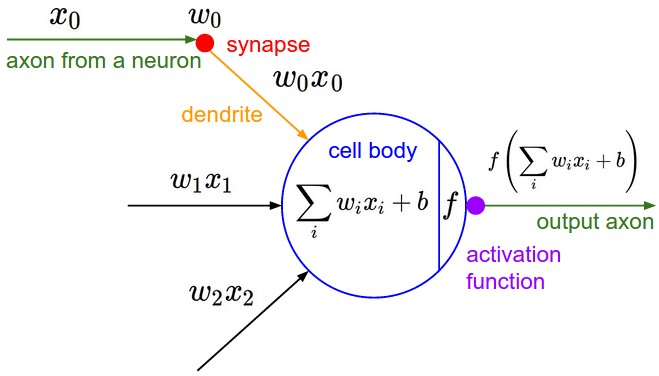
\includegraphics[width=0.4\textwidth]{Images/nn/1.jpeg}
  \caption{Cell diagram}
\end{figure}

An example code for forward-propagating a single neuron might look as follows:


\begin{lstlisting}[frame=single]
class Neuron(object):
  # ... 
  def forward(inputs):
    """ assume inputs and weights are 1-D numpy arrays and bias is a number """
    cell_body_sum = np.sum(inputs * self.weights) + self.bias
    firing_rate = 1.0 / (1.0 + math.exp(-cell_body_sum)) # sigmoid activation function
    return firing_rate
\end{lstlisting}

In other words, each neuron performs a dot product with the input and its weights, adds the bias and applies the non-linearity (or activation function), in this case the sigmoid $\sigma(x)=1/(1+e^{−x})$. We will go into more details about different activation functions at the end of this section.

\subsection*{Single neuron as a linear classifier}

The mathematical form of the model Neuron’s forward computation might look familiar to you. As with linear classifiers, a neuron has the capacity to ``like” (activation near one) or ``dislike” (activation near zero) certain linear regions of its input space. Hence, with an appropriate loss function on the neuron’s output, we can turn a single neuron into a linear classifier:

\paragraph*{Binary Softmax classifier} For example, we can interpret $\sigma(\sum_iw_ix_i+b)$ to be the probability of one of the classes $P(y_i=1∣x_i;w)$. The probability of the other class would be $P(y_i=0∣x_i;w)=1−P(y_i=1∣x_i;w)$, since they must sum to one. With this interpretation, we can formulate the cross-entropy loss as we have seen in the Linear Classification section, and optimizing it would lead to a binary Softmax classifier (also known as logistic regression). Since the sigmoid function is restricted to be between 0-1, the predictions of this classifier are based on whether the output of the neuron is greater than 0.5.

\paragraph*{Binary SVM classifier} Alternatively, we could attach a max-margin hinge loss to the output of the neuron and train it to become a binary Support Vector Machine.

\paragraph*{Regularization interpretation} The regularization loss in both SVM/Softmax cases could in this biological view be interpreted as gradual forgetting, since it would have the effect of driving all synaptic weights $w$ towards zero after every parameter update.

\subsection*{Layer-wise organization}
Neural Networks as neurons in graphs. Neural Networks are modeled as collections of neurons that are connected in an acyclic graph. In other words, the outputs of some neurons can become inputs to other neurons. Cycles are not allowed since that would imply an infinite loop in the forward pass of a network. Instead of an amorphous blobs of connected neurons, Neural Network models are often organized into distinct layers of neurons. For regular neural networks, the most common layer type is the \textbf{fully-connected layer} in which neurons between two adjacent layers are fully pairwise connected, but neurons within a single layer share no connections. 

\begin{figure}[h]
  \centering
  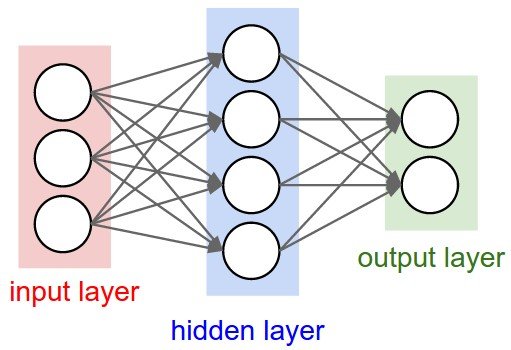
\includegraphics[width=0.3\textwidth]{Images/nn/2.jpeg}
  \caption{Layer-wise organization. A 2-layer Neural Network (one hidden layer of 4 neurons (or units) and one output layer with 2 neurons), and three inputs}
\end{figure}

\subsection*{Example feed-forward computation}
\begin{lstlisting}[frame=single]
# forward-pass of a 3-layer neural network:
f = lambda x: 1.0/(1.0 + np.exp(-x)) # activation function (use sigmoid)
x = np.random.randn(3, 1) # random input vector of three numbers (3x1)
h1 = f(np.dot(W1, x) + b1) # calculate first hidden layer activations (4x1)
h2 = f(np.dot(W2, h1) + b2) # calculate second hidden layer activations (4x1)
out = np.dot(W3, h2) + b3 # output neuron (1x1)
\end{lstlisting}


\subsection*{Setting number of layers and their sizes}
How do we decide on what architecture to use when faced with a practical problem? Should we use no hidden layers? One hidden layer? Two hidden layers? How large should each layer be? First, note that as we increase the size and number of layers in a Neural Network, the capacity of the network increases. That is, the space of representable functions grows since the neurons can collaborate to express many different functions. For example, suppose we had a binary classification problem in two dimensions. We could train three separate neural networks, each with one hidden layer of some size and obtain different classifiers (Fig. \ref{fig:nn_classifiers}).

\begin{figure}[h]
  \centering
  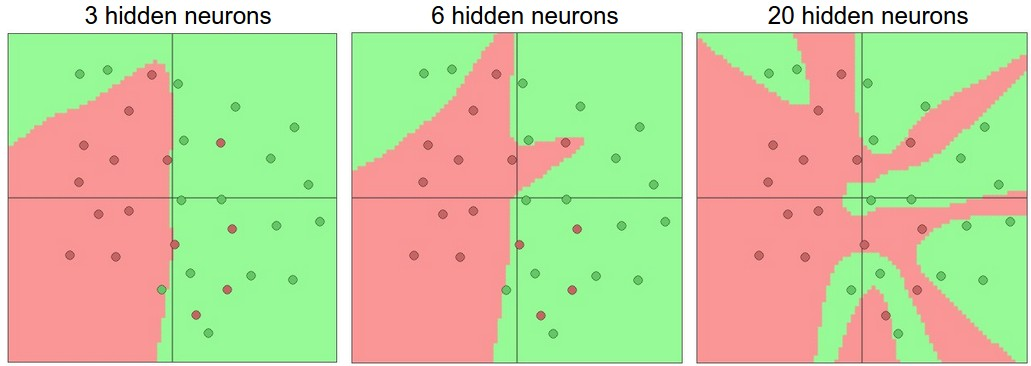
\includegraphics[width=0.6\textwidth]{Images/nn/3.jpeg}
  \caption{Larger Neural Networks can represent more complicated functions. You can play with these examples in \href{http://cs.stanford.edu/people/karpathy/convnetjs/demo/classify2d.html}{this ConvNetsJS demo}.}
  \label{fig:nn_classifiers}
\end{figure}

In the diagram above, we can see that Neural Networks with more neurons can express more complicated functions. However, this is both a blessing (since we can learn to classify more complicated data) and a curse (since it is easier to overfit the training data). \textbf{Overfitting} occurs when a model with high capacity fits the noise in the data instead of the (assumed) underlying relationship. For example, the model with 20 hidden neurons fits all the training data but at the cost of segmenting the space into many disjoint red and green decision regions. The model with 3 hidden neurons only has the representational power to classify the data in broad strokes. It models the data as two blobs and interprets the few red points inside the green cluster as \textbf{outliers} (noise). In practice, this could lead to better \textbf{generalization} on the test set. To reiterate, the \textbf{regularization} strength is the preferred way to control the overfitting of a neural network. We can look at the results achieved by three different settings (Fig. \ref{fig:nn_reg}).

\begin{figure}[h]
  \centering
  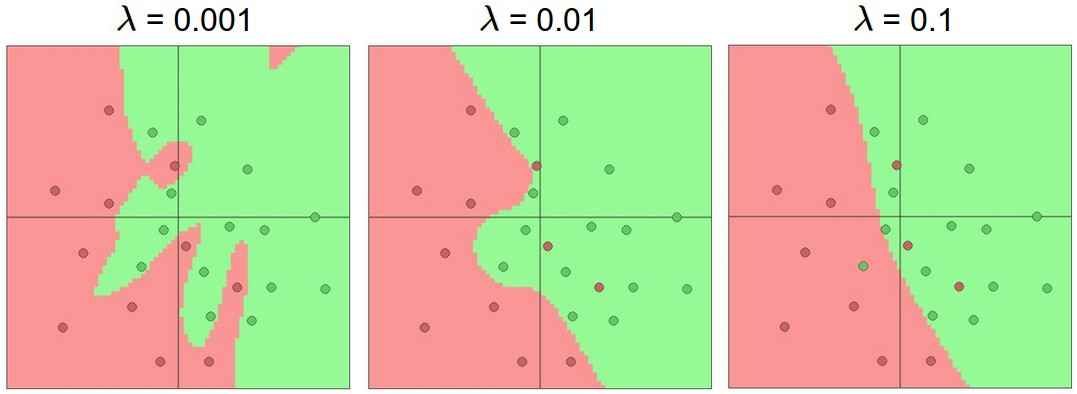
\includegraphics[width=0.6\textwidth]{Images/nn/4.jpeg}
  \caption{The effects of regularization strength: Each neural network above has 20 hidden neurons, but changing the regularization strength makes its final decision regions smoother with a higher regularization. You can play with these examples in \href{http://cs.stanford.edu/people/karpathy/convnetjs/demo/classify2d.html}{this ConvNetsJS demo}.}
    \label{fig:nn_reg}
\end{figure}